\documentclass[10pt,oneside,slovak,a4paper]{article}
\usepackage[slovak]{babel}
\usepackage[IL2]{fontenc}
\usepackage[utf8]{inputenc}
\usepackage{graphicx}
\usepackage{url} 
\usepackage{hyperref} 
\usepackage{cite}
\usepackage{float}



\title{Načo je Autodesk Maya?\thanks{Semestrálny projekt v predmete Metódy inžinierskej práce, ak. rok 2020/21, vedenie: Ing. Fedor Lehocki, PhD.}}

\author{Hieu Le Minh\\[2pt]
	{\small Slovenská technická univerzita v Bratislave}\\
	{\small Fakulta informatiky a informačných technológií}\\
	{\small \texttt{xleminhh@stuba.sk}}
	}

\date{\small 5. november 2021}



\begin{document}

\maketitle

\begin{abstract}
Ja som si vybral na rámcovú tému modelovanie v softvérovom inžinierstve program Autodesk Maya
- je to program využívaný na vytváranie 3D animácií. 
Plánujem sa hlavne zamerať na opis tohto programu, ako funguje, kde sa používa, v akom 
programovacom jazyku sa píše a tak ďalej. Rád by som ešte spomenul výhody a nevýhody, či 
sa tento program oplatí používať a na to by som potom nadviazal porovnanie s inými populárnymi programami na animácie.
\end{abstract}



\section{Úvod}

Hovorí sa, že nikto nie je príliš starý na rozprávky a hry. Ešte doteraz si rád pozriem nejakú tú rozprávku alebo zahrám hry. V poslednej dobe niekedy uvažujem pri tom čo pozerám ako dlho muselo trvať spracovanie alebo čo sa muselo použiť na spracovanie takéhoto niečoho. Preto som si vybral rámcovú tému Autodesk Maya. Celkom ma zaujalo, ako je možné vytvárať niektoré animácie pomocou tohto softvéru, tak som sa vydal na cestu hľadania odpovedí a rozhodol som sa ich s Vami zdieľať.

Tu je explicitná štruktúra článku.
Autodesk Maya softvér je vysvetlený v tejto časti.~\ref{AM}.
Vysvetlenie MEL a Python.~\ref{python}.
Výhody a nevýhody používania tohto programu sa nachádza tu.~\ref{vyhnevyh}.
Porovnanie Maya a Blender.~\ref{porovnanie}.
Použitie Unity 3D a Maya.~\ref{3d}.
Záverečné poznámky prináša časť~\ref{zaver}.



\section{Autodesk Maya - čo to vôbec je?} \label{AM}

Autodesk Maya je program, ktorý umožňuje 3D animovanie, modelovanie, simulácie, vykresľovanie a ďalšie. Je všestranný a mnohí ho považujú za priemyselný štandard pre animácie. Veľa známych filmových štúdií používa Autodesk Maya ako sú napríklad Blue Sky Studios, Framestore, Moving Picture Company. Tento softvér bol použitý na animovanie známych a ocenených filmových rozprávok ako sú „Frozen“ a „Wreck It Ralph“.\\

Pomocou Maya môžete vytvárať 3D prvky pre filmy, seriály a dokonca aj pre videohry. Zahŕňa niekoľko rôznych komponentov umenia vrátane vytvárania 3D modelov, zostavovania postavy, animácií, dynamiky, osvetlenia a vykresľovania. Maya obsahuje ľahko použiteľné nástroje na zjednodušenie všetkých týchto úloh.\\

Autodesk Maya je dostupný pre operačné systémy Windows, Mac a Linux. Na 1 rok Vás bude tento program stáť 1700 dolárov, čo je v prepočte okolo 1500 eúr.



\section{MEL a Python} \label{python}
\paragraph{MEL}
celým názvom Maya Embedded Language je skriptový jazyk. Funkcie ako menu, buttony a mnohé iné, ktoré sa v programe nachádzajú, sú napísane cez tento MEL.
\paragraph{Python}
patrí do rebríčka jedných z najpopulárnejších a najobľúbenejších programovacích jazykov. Používa sa napríklad na výrobu rôznych hier, programov a aj na umelú inteligenciu.\\

Prečo som tu spomenul python? MEL je hlavný jazyk programu Autodesk Maya, ale tento program taktiež podporuje písanie v pythone. Výhoda v používaní pythonu je tá, že python narozdiel od MEL má možnosť class managementu, taktiež je štruktúra kódu ľahšie čítateľná a zrozumiteľná. MEL má iba funkcie, ktoré súvisia s Mayou narozdiel od pythonu, ktorý je široko podporovaný rôznymi softvérami.\cite{evaluationmaya}



\section{Výhody a nevýhody} \label{vyhnevyh}
Tu by som rád spomenul niektoré výhody a nevýhody tohto softvéru.

\paragraph{Výhody}
\begin{itemize}
\item umožňuje používateľom pracovať rýchlejšie a efektívnejšie
\item dokončená práca sa dá rýchlejšie kontrolovať\cite{educbaa2021}
\item poskytuje veľa funkcií
\item vytvára dobré rendre
\end{itemize}

\paragraph{Nevýhody}
\begin{itemize}
\item potrebuje veľa času na rendrovanie
\item pre začiatočníkov celkom náročné na používanie
\item niekedy crashuje
\item drahé
\end{itemize}

\section{Porovnanie Maya a Blender} \label{porovnanie}

Vybral som na porovnanie Blender, pretože tieto 2 softvéri sú navonok veľmi podobné. Dovolím si Vám v nasledujúcich bodoch ukázať, čo majú spoločné a čo rozdielne.

\begin{itemize}
\item spoločné
	\begin{itemize}
	\item sú podobné, pretože obe sa použivajú na animovanie
	\item dajú sa použiť na operačných systémoc Windows, Mac OS a Linux
	\end{itemize}

\item rozdielne
	\begin{itemize}
	\item ako som už v úvode spomínal, za použivanie Maya musíte platiť, zatial čo Blender je zadarmo, lebo je open-source
	\item Maya je viac komplikovaná na používanie ako Blender (pre začiatočníkov)
	\item Maya je určená skôr väčším firmám, Blender je zas skôr určený pre start-upy alebo začiatočníkom
	\item za používanie Maya sa platí, takže je výkonnejšia ako Blender a má menej bugov\cite{educba2021}
	\end{itemize}
\end{itemize}



\section{Použitie Unity 3D a Maya} \label{3d}

Na to aby sme mohli pokračovať v tejto téme, tak Vám najprv vysvetlím čo je Unity 3D.\\

\emph{Unity 3D} je softvér, ktorý poháňa celý program, je to niečo ako motor. Jeden z naoblúbenejších softvérov na trhu. Je jednoduchý na používanie a nemusíte za to nič platiť. Oblúbený, pretože umožňuje programátorom písať v C\texttt{\#} alebo JavaScript. Taktiež má vbudovaný Visual Studio, čiže kód bude prehľadný a ľahšie čítateľný. Ponúka Vám aj nástroje na animácie, aby ste mohli vytvárať Vaše nie len 3D animácie, ale aj 2D.\\

Prečo Unity 3D a Maya? Dôvodom je, že Unity 3D chýba modelovacie schopnosti a v tomto to Maya dopĺňa.\cite{labschutz2011content}\\

Príklad:
Keďže počet prípadov, kde deti s ADHD (porucha pozornosti s hyperaktivitou), dislexiou, disgrafiou a ďaľšími neschopnosťami narastá, vytvorila sa aplikácia pomocou Maya a Unity, ktorá sa volá "Learning Disability Application". Z názvu je už jasné, že sa to bude zaoberať nejakými neschopnosťami alebo postihnutiami. Je to hra/aplikácia určená pre učiteľov, ktorí sa môžu otestovať a dokonca aj naučiť ako sa zachovať a čo robiť, ak búdu mať takého študenta. Hra ich prevedie reálnymi situáciami, 2 scenáriami (scenário 1 ~\ref{f:scenario1} a scenário 2 ~\ref{f:scenario2}), ktoré môžu nastať a nakonci sú učitelia evaluovaný buď "right decision" (správna voľba) alebo "wrong decision" (nesprávna voľba)\cite{studies}.

\begin{figure*}[h]
\centering
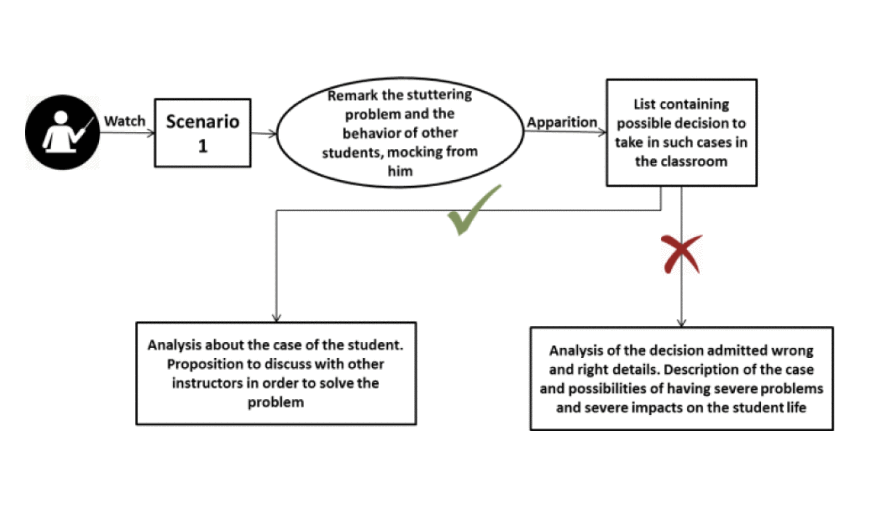
\includegraphics[scale=0.37]{scenario 1.png}
\caption{scenário 1\cite{studies}}
\label{f:scenario1}
\end{figure*}
\begin{figure*}[h]
\centering
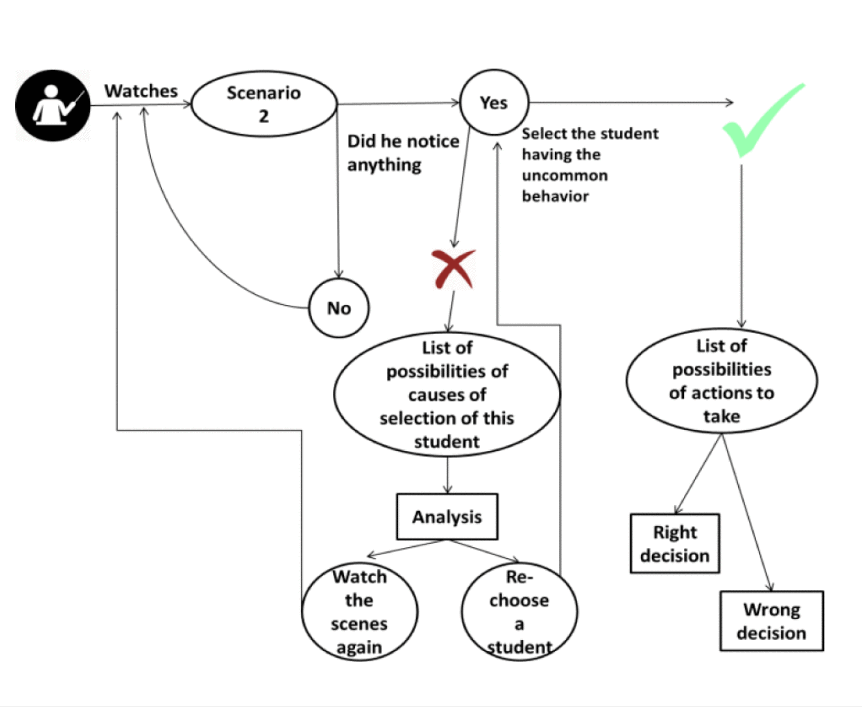
\includegraphics[scale=0.37]{scenario 2.png}
\caption{scenário 2\cite{studies}}
\label{f:scenario2}
\end{figure*}





\section{Záver} \label{zaver}

V tomto článku som sa snažil Vás oboznámiť so základnými informáciami o Autodesk Maya. Prešli sme od témy kde som Vám vysvetloval čo to je Autodesk Maya až po vytvorenie aplikácie pomocou nej. Tento softvér je hlavne určený pre animátorov a dizajnérov. Ako som už spomínal, neradím Vám použivať tento softvér ak ste nováčik v tomto odbore, kvôli náročnosti a taktiež aby ste nemiňali len tak Vaše peniaze, lebo Maya nie je zadarmo. Je to veľmi dobrý softvér, ktorý si veľa používateľov pochvaľuje. 

\bibliography{literatura.bib}
\bibliographystyle{plain} 
\end{document}
